\documentclass[16 pt]{amsart}
\usepackage{amscd,amsmath,amsthm,amssymb}
\usepackage{enumerate,varioref}
\usepackage{epsfig}
\usepackage{graphicx}
\usepackage{mathtools}
\usepackage{svg}
\usepackage{tikz}
\usetikzlibrary{automata,positioning}
\newtheorem{thm}{Theorem}
\newtheorem{cor}[thm]{Corollary}
\newtheorem{lem}[thm]{Lemma}
\newtheorem{prop}[thm]{Proposition}
\theoremstyle{definition}
\newtheorem{defn}[thm]{Definition}
\theoremstyle{remark}
\newtheorem{ex}[thm]{Example}
\newtheorem{rem}[thm]{Remark}
\numberwithin{equation}{subsection}
\newcommand{\R}{\mathbb{R}}
\newcommand{\Z}{\mathbb{Z}}
\newcommand{\C}{\mathbb{C}}
\newcommand{\Q}{\mathbb{Q}}
\newcommand{\lh}{\lim_{h\rightarrow 0}}
\begin{document}

\title{Homework Solutions and Notes\\ 
Maths 141 Winter 2017}
\maketitle 



\section{Problems}

1.1:  (a) Negate the following statement:
\[
\forall x\in \R_+, \exists y \in \Z_+ \text{ s.t. } y<x^2  
\]


Solution: 
\[
\exists x\in\R_+ \text{ so that } \forall y\in\Z_+, y\ge x^2
\]


(b) Found a counterexample to show that the above statement is false. 

We need to find an $x$ where no matter which positive $y$ we choose $y\ge x^2$.  We need to choose $x$ so that $x^2<1.$  Let's pick $x=1/2$.\\

1.2.  Prove the following summations by induction.  You may use $n=0$ as the base case for each of the following:\\

(a) 
\[
\sum_{k=0}^{n} k^2 = \frac{n(n+1)(2n+1)}{6}
\]

Base case $(n=0)$  
\[
0^2 = \frac{0(1)(1)}{6}
\]
which checks out.  Now assume for some $m\ge 0$.

\[
\sum_{k=0}^{m} k^2 = \frac{m(m+1)(2m+1)}{6}
\]

Then we need to show for this $m$

\[
\sum_{k=0}^{m+1} k^2 = \frac{(m+1)(m+2)(2m+3)}{6}
\]

So we compute:
\begin{eqnarray}
\sum_{k=0}^{m+1} k^2 & = & \sum_{k=0}^m k^2 + (m+1)^2\nonumber \\
& = & \frac{m(m+1)(2m+1)}{6} + (m+1)^2 \nonumber \\
& = & \frac{(m+1)}{6} (m(2m+1) + 6(m+1)\nonumber\\
& = & \frac{(m+1)}{6}(2m^2 + 7m + 6)\nonumber \\
& = & \frac{(m+1)(m+2)(2m+3)}{6} \nonumber
\end{eqnarray}


(b) 
\[
\sum_{k=0}^{n} k^3 = \left(\frac{n(n+1)}{2}\right)^2
\]


(Base case $n=0$) $0^3 = \left(\frac{0(1)}{2}\right)^2$ which checks out.  Now assume for some $m\ge0$

\[
\sum_{k=0}^{m} k^3 = \left(\frac{m(m+1)}{2}\right)^2
\]
and we wish to show
\[
\sum_{k=0}^{m+1} k^3 = \left(\frac{(m+1)(m+2)}{2}\right)^2
\]

We compute
\begin{eqnarray}
\sum_{k=0}^{m+1} k^3 & = & \sum_{k=0}^{m} k^3 + (m+1)^3 \nonumber \\
& = & \left(\frac{m(m+1)}{2}\right)^2 + (m+1)^3 \nonumber \\
& = & \left(\frac{(m+1)}{2}\right)^2 (m^2 + 4(m+1))\nonumber \\
& = & \left(\frac{(m+1)(m+2)}{2}\right)^2. \nonumber
\end{eqnarray}


(c) 
\[
\sum_{j=0}^{n} 2^j = 2^{n+1}-1
\]


(Base case $n=0$) $2^0 = 2^1-1$ which checks out.  Now we assume for some $m\ge 0$

\[
\sum_{j=0}^{m} 2^j = 2^{m+1}-1
\]
and we wish to show
\[
\sum_{j=0}^{m+1} 2^j = 2^{m+2}-1
\]

We compute
\begin{eqnarray}
\sum_{j=0}^{m+1} 2^j & = & \sum_{j=0}^{m} 2^j + 2^{m+1} \nonumber\\
& = & 2^{m+1}-1 + 2^{m+1} \nonumber\\
& = & 2^{m+2} - 1. \nonumber
\end{eqnarray}

(d)
\[
\sum_{j=0}^{n} r^j = \left(\frac{r^{n+1}-1}{r-1}\right)
\]


(Base case $n=0$) $r^0 = \frac{r-1}{r-1}$ so long as $r\ne0,1$  Now we assume for some $m\ge 0$

\[
\sum_{j=0}^{m} r^j = \left(\frac{r^{m+1}-1}{r-1}\right)
\]

and we wish to show

\[
\sum_{j=0}^{m+1} r^j = \left(\frac{r^{m+2}-1}{r-1}\right)
\]


We compute
\begin{eqnarray}
\sum_{j=0}^{m+1} r^j & = & \sum_{j=0}^{m}r^j + r^{m+1}\nonumber \\
& = & \left(\frac{r^{m+1}-1}{r-1}\right) + r^{m+1} \nonumber\\
& = & \frac{r^{m+1}-1 + (r-1)r^{m+1}}{r-1} \nonumber\\
& = & \frac{r^{m+2}-1}{r-1}\nonumber.
\end{eqnarray}


(e)
\[
\sum_{k=0}^n (-1)^k = \frac{1}{2}(1+(-1)^n)
\]

(Base case $n=0$) $(-1)^0 = \frac{1}{2}(1+(-1)^0)$ which checks out.  Now we assume for some $m\ge 0$

\[
\sum_{k=0}^m (-1)^k = \frac{1}{2}(1+(-1)^m)
\]
 and we wish to show
 \[
 \sum_{k=0}^{m+1} (-1)^k = \frac{1}{2}(1+(-1)^{m+1})
 \]

We compute
\begin{eqnarray}
 \sum_{k=0}^{m+1} (-1)^k & = &  \sum_{k=0}^{m} (-1)^k + (-1)^{m+1}\nonumber \\
 & = & \frac{1}{2}(1+(-1)^m) + (-1)^{m+1}\nonumber \\
 & = & \frac{1}{2}(1+(-1)^m + 2(-1)^{m+1}) \nonumber \\
 & = & \frac{1}{2}(1 + (-1)^m(1-2))\nonumber\\
 & = & \frac{1}{2}(1+(-1)^{m+1})\nonumber
\end{eqnarray}

1.3. Prove the following product formulas by induction.  You may assume the lower index to be the base case in all problems.\\

(a) 
\[
\prod_{k=2}^{n} \left(1 - \frac{1}{k^2}\right) = \frac{n+1}{2n}
\]

(Base case $n=2$) $\left(1 - \frac{1}{2^2}\right) = \frac{2+1}{2(2)}$ which check out. Now we assume for some $m\ge2$

\[
\prod_{k=2}^{m} \left(1 - \frac{1}{k^2}\right) = \frac{m+1}{2m}
\]
and we wish to show
\[
\prod_{k=2}^{m+1} \left(1 - \frac{1}{k^2}\right) = \frac{m+2}{2(m+1)}
\]

We compute
\begin{eqnarray}
\prod_{k=2}^{m+1} \left(1 - \frac{1}{k^2}\right) & = & \prod_{k=2}^{m} \left(1 - \frac{1}{k^2}\right)*\left(1 - \frac{1}{(m+1)^2}\right) \nonumber \\
& = & \left(\frac{m+1}{2m}\right)*\left(1 - \frac{1}{(m+1)^2}\right)\nonumber \\
& = & \left(\frac{m+1}{2m}\right)*\left(\frac{(m+1)^2-1}{(m+1)^2}\right)\nonumber\\
& = & \left(\frac{m(m+2)}{2m(m+1)^2}\right)\nonumber \\
& = & \frac{m+2}{2(m+1)} \nonumber
\end{eqnarray}


(b) 
\[
\prod_{j=1}^{n} (2j-1) = \frac{(2n)!}{2^n n!}
\]

(Base case $n=1$) $(2-1) = \frac{2!}{2 * 1!}$ which checks out.  Now we assume for some $m\ge 1$

\[
\prod_{j=1}^{m} (2j-1) = \frac{(2m)!}{2^m m!}
\]

and we wish to show

\[
\prod_{j=1}^{m+1} (2j-1) = \frac{(2(m+1))!}{2^(m+1) (m+1)!}
\]


We compute
\begin{eqnarray}
\prod_{j=1}^{m+1} (2j-1) & = & \prod_{j=1}^{m} (2j-1) * (2m+1)\nonumber \\
& = & \frac{(2m)!}{2^m m!} * (2m+1) \nonumber \\
& = & \frac{(2m)!}{2^m m!} * (2m+1) * \frac{2m+2}{2m+2} \nonumber \\
& = & \frac{(2m+2)!}{2^{m+1}(m+1)!} \nonumber
\end{eqnarray}

(c)
\[
\prod_{k=1}^{n} i^k = i^{\binom{n+1}{2}}
\]


Base case $n=1$ $i^1= i^{\binom{2}{2}}$


Induction assume at some $m\ge 1$ 
\[
\prod_{k=1}^{m} i^k = i^{\binom{m+1}{2}}
\]

Show for $m+1$

\[
\prod_{k=1}^{m+1} i^k = i^{\binom{m+2}{2}}
\]

We compute
\begin{eqnarray}
\prod_{k=1}^{m+1} i^k &=& \prod_{k=1}^{m}i^k * i^{m+1}\nonumber \\
&=&  i^{\binom{m+1}{2}}* i^{m+2}\nonumber\\
& = & i^{\binom{m+2}{2}} \nonumber
\end{eqnarray}

1.4.  For every $n>1$ prove the following inequality

\[
\sqrt{n} < \sum_{k=1}^{n} \frac{1}{\sqrt{k}}
\]

In this case we check the base slightly differently:
\[
\sqrt{2} < 1 + \frac{1}{\sqrt{2}}  \iff 2 < \sqrt{2} +1
\]
This is true since $1<\sqrt{2}$.

Now for the inductive assumption, we assume for some $m\ge 2$ that

\[
\sqrt{m} < \sum_{k=1}^{m} \frac{1}{\sqrt{k}}
\]

We wish to show
\[
\sqrt{m+1} < \sum_{k=1}^{m+1} \frac{1}{\sqrt{k}}
\]


In this case we see from our assumption that
\[
\sqrt{m} + \frac{1}{\sqrt{m+1}} < \sum_{k=1}^{m} \frac{1}{\sqrt{k}} + \frac{1}{\sqrt{m+1}}
\]

So if we can fit $\sqrt{m+1}$ on the left then we appeal to transitivity of $<$ and we only need to show
\[
\sqrt{m+1} < \sqrt{m} + \frac{1}{\sqrt{m+1}}
\]

Clear the denominators and subtract one to achieve
\[
m+1 < \sqrt{m(m+1)} + 1 \implies m < \sqrt{m(m+1)}
\]

Squaring both sides we have
\[
m^2 < m^2 + m
\]
since $m\ge 2$ this holds.\\



1.5. Let $x,y$ be nonzero integers and let $n$ be a positive integer.  Prove the following by induction.

\[
(x-y) | (x^n - y^n)
\]

The base case is easy since $(x-y)|0$ is always true.
Now assume that $(x-y)|(x^k-y^k)$ for some $k>0$ then we have the following
\begin{eqnarray}
(x-y)|(x^k-y^k) & \implies & (x-y)| x(x^k-y^k) \\
(x-y)|(x-y) & \implies & (x-y)|(x-y)y^k\\
\end{eqnarray}

Adding the two right hand multiples we have
\[
(x-y) | (x(x^k-y^k) + (x-y)y^k) \implies (x-y)|(x^{k+1}-y^{k+1})
\]


2.1.  Prove for the following by induction for $n>10$.

\[
\frac{n^n}{3^n} < n! < \frac{n^n}{2^n}
\]

Hint:  In this problem we're really solving two different problems.  Consider each inequality separately.  You will find the following inequality to be helpful.  You may take this to be true.  If you need more documentation or further explanation, read some information about $e$.

\[
2\le \left( 1+ \frac{1}{n}\right)^n < 3.
\]

Let's solve the righthand inequality first.  The base case we can check by computing directly.  For the inductive step we assume for some $k>10$
\[
k! < \frac{k^k}{2^k} \iff 2^k k! < k^k
\]

We'll use the multiplicative form and we wish to show
\[
2^{k+1}(k+1)! < (k+1)^{(k+1)}
\]


As with 1.4 we want to sandwich something in the middle of this inequality and use transitivity.
First, if we multiply the assumption by 2 we get
\[
2^{k+1} k! < 2k^k
\]

Additionally the goal is equivalent (by canceling one copy of $k+1$) to
\[
2^{k+1} k! < (k+1)^k 
\]

So we wish to show
\[
2k^k < (k+1)^k \iff 2 < \left(\frac{k+1}{k}\right)k 
\]

This is, of course, the hint given.  Now let's look at the inductive case for the other inequality. We want to show

\[
(k+1)^k < 3 k^k 
\]

Again, dividing we get
\[
\left(\frac{k+1}{k}\right)^k < 3.
\]






2.2.  Let $p>2$ be a prime number and let $a\ge 1$.  

\[
p | (a^p-a).
\]

(a) What is the induction variable?  Hint: It's not $p$.\\

We're inducting on $a$ since $p$ is some fixed prime.



(b) Write the binomial expansion of $(a+1)^p$.\\


The binomial expansion is
\[
(a+b)^p = \sum_{k=0}^{p}\binom{p}{k}a^{p-k}b^k
\]

When $b=1$ we get

\[
(a+1)^p = \sum_{k=0}^{p}\binom{p}{k}a^{p-k}
\]




(c) Why does $p| \binom{p}{k}$ for every $1<k<p$?\\

Consider the fact that $p$ is prime and that $\binom{p}{k}$ is a positive integer. Every number in the denominator is smaller than $p$ and thus does not divide $p$.  So in this case we have $\binom{p}{k} = p*m$ for some $m\in \Z$.  Basically, it's because $p$ is prime.  Let's take an easy example when $p$ is not prime.

\[
4 \not| \binom{4}{2} 
\]


(d) Prove the divisibility by induction.


Now assume $p | (a^p-a)$ let's show that
\[
p | (a+1)^p-(a+1)
\]

Expanding we have
\[
(a+1)^p - (a+1) = (a^p-a)+ \sum_{k=1}^{p-1}\binom{p}{k}a^{p-k}
\]

Now $p$ divides the first term by assumption and the sum since it divides each binomial coefficient (since $p$ is prime).





2.3.  Let $a,b\in \R$ and $n\in \mathbb{N}$.  Prove the following by induction:

\[
\begin{bmatrix}
a & b \\
0 & a
\end{bmatrix}^n = \begin{bmatrix}
a^n & nba^{n-1}\\
0 & a^n
\end{bmatrix}
\]



Base case $n=1$

\[
\begin{bmatrix}
a & b \\
0 & a
\end{bmatrix}^1 = \begin{bmatrix}
a^1 & 1ba^{1-1}\\
0 & a^1
\end{bmatrix}
\]
which checks out.  Now assume
\[
\begin{bmatrix}
a & b \\
0 & a
\end{bmatrix}^k = \begin{bmatrix}
a^k & kba^{k-1}\\
0 & a^k
\end{bmatrix}
\]

Show

\[
\begin{bmatrix}
a & b \\
0 & a
\end{bmatrix}^{k+1} = \begin{bmatrix}
a^{k+1} & (k+1)ba^{k}\\
0 & a^{k+1}
\end{bmatrix}
\]


We compute
\begin{eqnarray}
\begin{bmatrix}
a & b \\
0 & a
\end{bmatrix}^{k+1} & = & 
\begin{bmatrix}
a & b \\
0 & a
\end{bmatrix}^{k}*
\begin{bmatrix}
a & b \\
0 & a
\end{bmatrix} \nonumber \\
& = & 
\begin{bmatrix}
a^k & kab^{k-1} \\
0 & a^k
\end{bmatrix}*
\begin{bmatrix}
a & b \\
0 & a
\end{bmatrix} \nonumber \\
& = &
\begin{bmatrix}
a^k *a & a^k*b + kba^{k-1}*a \\
0 & a^k * a
\end{bmatrix} \nonumber \\
& = & 
\begin{bmatrix}
a^{k+1} & (k+1)ba^k \\
0 & a^{k+1}
\end{bmatrix} \nonumber
\end{eqnarray}





2.4.  Define the Fibonacci numbers by $F_{n+1} = F_n + F_{n-1}$ with the first two numbers $F_0 = 0, F_1=1$.\\

(a) Prove $F_n < 2^n$ for every $n>0$.\\


In the base cases
\[
F_0 = 0< 2^0, F_1 = 1 < 2^1
\]


Now we assume
\[
F_k<2^k \text{ and } F_{k-1}< 2^{k-1}
\]

Then we have

\[
F_{k+1} = F_k + F_{k-1} = 2^k + 2^{k-1} < 2^{k+1}
\]


(b) For every $n>0$ prove the following by induction:
\[
\begin{bmatrix}
1 & 1 \\
1 & 0
\end{bmatrix}^n = \begin{bmatrix}
F_{n+1} & F_n\\
F_n & F_{n-1}
\end{bmatrix}
\]


In the base case $n=1$
\[
\begin{bmatrix}
1 & 1\\
1 & 0
\end{bmatrix}^1 = \begin{bmatrix}
F_2 & F_1 \\
F_1 & F_0
\end{bmatrix}
\]


Now we assume

\[
\begin{bmatrix}
1 & 1 \\
1 & 0
\end{bmatrix}^k = \begin{bmatrix}
F_{k+1} & F_k\\
F_k & F_{k-1}
\end{bmatrix}
\]


and we wish to show

\[
\begin{bmatrix}
1 & 1 \\
1 & 0
\end{bmatrix}^{k+1} = \begin{bmatrix}
F_{k+2} & F_{k+1}\\
F_{k+1} & F_{k}
\end{bmatrix}
\]

We compute
\begin{eqnarray}
\begin{bmatrix}
1 & 1\\
1 & 0
\end{bmatrix}^{k+1} 
& = & 
\begin{bmatrix}
1 & 1\\
1 & 0
\end{bmatrix}^{k} *
\begin{bmatrix}
1 & 1\\
1 & 0
\end{bmatrix} \nonumber\\
& = & 
\begin{bmatrix}
F_{k+1} & F_k\\
F_k & F_{k-1}
\end{bmatrix} * 
\begin{bmatrix}
1 & 1\\
1 & 0
\end{bmatrix} \nonumber \\
& = &
\begin{bmatrix}
F_{k+1} + F_k & F_{k+1}\\
F_k + F_{k-1 }& F_{k}
\end{bmatrix}   \nonumber \\
& = & 
\begin{bmatrix}
F_{k+2} & F_{k+1}\\
F_{k+1} & F_{k}
\end{bmatrix} 
\end{eqnarray}




2.5.  In this problem we'll begin exploring some more advanced things we can do with matrices.  Of course, I'll provide the major mathematical components, and you'll prove them by induction.  A longer explanation will come in the notes at the end of this assignment.\\


Consider the following matrix:
\[
L = \begin{bmatrix}
2 & -1 & -1 \\
-1 & 1 & 0\\
-1 & 0 & 1
\end{bmatrix}
\]

This is another related matrix to a graph, called the Laplacian of a graph.

\[
L = \begin{bmatrix}
2 & 0 & 0\\
0 & 1 & 0\\
0 & 0 & 1
\end{bmatrix} - \begin{bmatrix}
0 & 1 & 1\\
1 & 0 & 0\\
1 & 0 & 0
\end{bmatrix} = D-A
\]

Where $D$ is the degree matrix and $A$ is the adjacency matrix which we've previously studied.

(a) Draw the graph associated with $A$.\\
\[
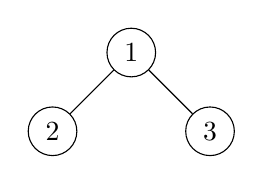
\begin{tikzpicture}
\node[circle, draw](1) at (1,1){1};
\node[circle, draw](2) at (0,0){2};
\node[circle, draw](3) at (2,0){3};
\foreach \from/\to in {1/2,1/3} 
\draw (\from) -- (\to);
\end{tikzpicture}
\]

(b) Show the 3 following equalities:
\[
L v_j = \lambda_j v_j
\]

where
\[
(\lambda_1,v_1) = \left(0, 
\begin{bmatrix}
1 \\ 1\\ 1
\end{bmatrix}\right), 
(\lambda_2,v_2) = \left(1, 
\begin{bmatrix}
0 \\ 1\\-1
\end{bmatrix}\right), 
(\lambda_3,v_3) = \left(3,
\begin{bmatrix}
2 \\ -1 \\ -1
\end{bmatrix}\right)
\]


In order to show this step, we simply multiply the given pairs:
\[
\begin{bmatrix}
2 & -1 & -1 \\
-1 & 1 & 0\\
-1 & 0 & 1
\end{bmatrix}  
\begin{bmatrix}
1\\1\\1
\end{bmatrix} = \begin{bmatrix}
0 \\ 0 \\ 0
\end{bmatrix} = 0\begin{bmatrix}
1\\1\\1
\end{bmatrix}
\]
\[
\begin{bmatrix}
2 & -1 & -1 \\
-1 & 1 & 0\\
-1 & 0 & 1
\end{bmatrix}  
\begin{bmatrix}
0\\1\\-1
\end{bmatrix} = \begin{bmatrix}
0 \\ 1 \\ -1
\end{bmatrix} = 1\begin{bmatrix}
0\\1\\-1
\end{bmatrix}
\]
\[
\begin{bmatrix}
2 & -1 & -1 \\
-1 & 1 & 0\\
-1 & 0 & 1
\end{bmatrix}  
\begin{bmatrix}
2\\-1\\-1
\end{bmatrix} = \begin{bmatrix}
6 \\ -3 \\ -3
\end{bmatrix} = 3\begin{bmatrix}
2\\-1\\-1
\end{bmatrix}
\]



(c) This leads us to the equality
\[
\begin{bmatrix}
2 & -1 & -1 \\
-1 & 1 & 0\\
-1 & 0 & 1
\end{bmatrix} = 
\begin{bmatrix}
1 & 0 & 2 \\
1 & 1 & -1\\
1 & -1 & -1
\end{bmatrix}
\begin{bmatrix}
0 & 0 & 0 \\
0 & 1 & 0\\
0 & 0 & 3
\end{bmatrix}
\begin{bmatrix}
1/3 & 1/3 & 1/3 \\
0 & 1/2 & -1/2\\
2/6 & -1/6 & -1/6
\end{bmatrix}
\]


Now verify

\[
\begin{bmatrix}
1 & 0 & 2 \\
1 & 1 & -1\\
1 & -1 & -1
\end{bmatrix}
\begin{bmatrix}
1/3 & 1/3 & 1/3 \\
0 & 1/2 & -1/2\\
2/6 & -1/6 & -1/6
\end{bmatrix}
=
\begin{bmatrix}
1 & 0 & 0\\
0 & 1 & 0\\
0 & 0 & 1
\end{bmatrix} = I
\]


This is called the $3\times 3$ identity matrix.\\

  

(d) Given any $3\times 3$ matrix $M$ show
\[
IM = MI = M
\]

(e) Now prove by induction (base case of $n=1$)

\[
\begin{bmatrix}
2 & -1 & -1 \\
-1 & 1 & 0\\
-1 & 0 & 1
\end{bmatrix}^n = 
\begin{bmatrix}
1 & 0 & 2 \\
1 & 1 & -1\\
1 & -1 & -1
\end{bmatrix}
\begin{bmatrix}
0 & 0 & 0 \\
0 & 1 & 0\\
0 & 0 & 3
\end{bmatrix}^n
\begin{bmatrix}
1/3 & 1/3 & 1/3 \\
0 & 1/2 & -1/2\\
2/6 & -1/6 & -1/6
\end{bmatrix}
\]

(f) Prove by induction, for any $\lambda_1,\lambda_2\lambda_3\in\R$

\[
\begin{bmatrix}
\lambda_1 & 0 & 0\\
0 & \lambda_2 & 0\\
0 & 0 & \lambda_3
\end{bmatrix}^n = 
\begin{bmatrix}
\lambda_1^n & 0 & 0\\
0 & \lambda_2^n & 0\\
0 & 0 & \lambda_3^n
\end{bmatrix}
\]


(g) In some ``well-behaved" cases we can compute functions of matrices (one of the main reasons we say matrices act like ``higher dimensional numbers") by making the function act on the middle diagonal matrix:  In our particular case

\[
f\left(\begin{bmatrix}
2 & -1 & -1 \\
-1 & 1 & 0\\
-1 & 0 & 1
\end{bmatrix}\right) = 
\begin{bmatrix}
1 & 0 & 2 \\
1 & 1 & -1\\
1 & -1 & -1
\end{bmatrix}
\begin{bmatrix}
f(0) & 0 & 0 \\
0 & f(1) & 0\\
0 & 0 & f(3)
\end{bmatrix}
\begin{bmatrix}
1/3 & 1/3 & 1/3 \\
0 & 1/2 & -1/2\\
2/6 & -1/6 & -1/6
\end{bmatrix}
\]

We've already proven by induction that this works for $f(x)=x^n$ when $n\in\mathbb{N}$.  Now let's have some ``fun".

Using this formula, compute:
\[
\cos(L),\sin(L)
\]

and show 
\[
\cos^2(L)+\sin^2(L) = I.
\]

\newpage

3.1.  Pell's equation is defined by considering a square free integer $n$.  The equation is
\[
x^2 - ny^2 = 1
\]

Geometrically this defines a hyperbola on which there are infinitely many points.  We, however, are interested in only the points $(x,y)$ where both are integers.  Additionally, since a hyperbola is symmetric about both major axes in the plane each solution $(x,y)$ actually defines 4 solutions.  For example:
\[
x^2 - 2y^2 =1
\]
Has solution $3^2 - 2 (2^2)=1$.  This could represent the solutions $(3,2),(-3,2),(3,-2),(-3,-2)$.  We'll only consider the solutions in the first quadrant for simplicity.  If Pell's equation has a solution then it has infinitely many solutions.  The solution which is closest to the origin is called the fundamental solution denoted $(x_1,y_1)$ (this will serve as our base case).  Consider then,
\[
(x^2-ny^2)^N = 1^N = 1
\]

So we will factor via a difference of squares.

\[
x^2 - n y^2 = (x + \sqrt{n}y)(x-\sqrt{n}y) = 1
\]

(a) Prove by induction that Pell's equation has infinitely many solutions defined by:
\[
x_k + \sqrt{n} y_k = (x_1+\sqrt{n}y_1)^k
\]


Solution: We define
\[
(x_1,y_1) \text{ is the fundamental solution}
\]

Now suppose 
\[
x_k^2- ny_k^2 = 1
\]

We want to show

\[
x_{k+1}^2- ny_{k+1}^2 = 1
\]


So let's compute:
\begin{eqnarray}
x_{k+1} + \sqrt{n} y_{k+1} & = & (x_1+\sqrt{n} y_1)^{k+1} \nonumber \\
& = & (x_k+\sqrt{n}y_k)(x_1 + \sqrt{n}y_1) \nonumber \\
& = & (x_k x_1 + ny_ky_1) + \sqrt{n}(x_ky_1 + y_kx_1)\nonumber
\end{eqnarray}

Which tells us
\[
x_{k+1} = x_kx_1 + ny_ky_1 \text{ and } y_{k+1} = x_ky_1 + y_kx_1
\]

So we compute
\begin{eqnarray}
x_{k+1}^2 - ny_{k+1}^2 & = & (x_kx_1 + ny_ky_1)^2 - n(x_ky_1 + y_kx_1)^2 \nonumber \\
& = & x_k^2x_1^2 + 2nx_1x_ky_1y_k + n^2y_k^2y_1^2 - n(x_k^2y_1^2 + 2x_1x_ky_1y_k + y_k^2x_1^2) \nonumber\\
& = & x_k^2(x_1^2-ny_1^2) - n y_k^2(x_1^2-ny_1^2) \nonumber \\
& = & x_k^2-ny_k^2 = 1 \nonumber
\end{eqnarray}


Hint: You will have to do some factoring here.\\

(b) We can convert this into a matrix equation:
\[
\begin{bmatrix}
x_{k+1}\\ y_{k+1}
\end{bmatrix} = 
\begin{bmatrix}
x_1 & ny_1\\
y_1 & x_1
\end{bmatrix}
\begin{bmatrix}
x_k \\ y_k
\end{bmatrix}
\]

Prove by induction:

\[
\begin{bmatrix}
x_{k+1}\\ y_{k+1}
\end{bmatrix} = 
\begin{bmatrix}
x_1 & ny_1\\
y_1 & x_1
\end{bmatrix}^k
\begin{bmatrix}
x_1 \\ y_1
\end{bmatrix}
\]


Solution:
\[
\begin{bmatrix}
x_2 \\ y_2
\end{bmatrix}
= 
\begin{bmatrix}
x_1 & ny_1 \\
y_1 & x_1
\end{bmatrix}
\begin{bmatrix}
x_1 \\y_1
\end{bmatrix}
\]

Now inductively

\[
\begin{bmatrix}
x_{k+1} \\ y_{k+1}
\end{bmatrix}
= 
\begin{bmatrix}
x_1 & ny_1 \\
y_1 & x_1
\end{bmatrix}
\begin{bmatrix}
x_k \\y_k
\end{bmatrix}
= 
\begin{bmatrix}
x_1 & ny_1\\
y_1 & x_1
\end{bmatrix}^k
\begin{bmatrix}
x_1 \\y_1
\end{bmatrix}
\]

(c) The fundamental solution for $n=2$ is $(3,2)$.  Compute the first 5 solutions for $n=2$.  What happens to the ratios
\[
\frac{x_1}{y_1},\frac{x_2}{y_2},\frac{x_3}{y_3},\frac{x_4}{y_4},\frac{x_5}{y_5},\dots?
\]

Let's check the ratios:
\[
\frac{3}{2},\frac{17}{12},\frac{99}{70}
\]

If we evaluate these numerically, we see that they converge to $\sqrt{2}$.

(d) the fundamental solution for $n=7$ is $(8,3)$.  Compute the first 5 solutions for $n=7$.  What happens to the ratios
\[
\frac{x_1}{y_1},\frac{x_2}{y_2},\frac{x_3}{y_3},\frac{x_4}{y_4},\frac{x_5}{y_5},\dots?
\]

(e) What is the fundamental solution for $n = m^2-1$, for some integer $m$?\\

The fundamental solution is $(m,1)$.


(f) Why do these ratios seem to converge?  Can you prove it?\\


Since $x_k$ and $y_k$ are growing the sum
\[
x_k + \sqrt{n}y_k 
\]
is growing faster.

That is
\[
(x_k-\sqrt{n}y_k)(x_k+\sqrt{n}y_k) = 1 \implies x_k-\sqrt{n}y_k = \frac{1}{x_k+\sqrt{n}y_k}
\]

This means $x_k \approx \sqrt{n} y_k$.

(Bonus): How fast do these ratios converge?\\



3.2.  Solve the recurrence relation with intial conditions $a_0 = 0, a_1 = 2$
\[
a_{n+2} - 3a_{n+1} + 3a_n = 0
\]

Solution: Let's get right to characteristic equation:
\[
r^2 - 3r + 3 = 0 \implies r = \frac{3 \pm \sqrt{9-12}}{2}
\]

So our general solution is
\[
a_n = A\left(\frac{3+\sqrt{-3}}{2}\right)^n + B\left(\frac{3-\sqrt{-3}}{2}\right)^n
\]

Now we solve with our initial conditions:
\[
a_0 = 0 = A+B \implies A=-B
\]

\[
a_1 = 2 = Ar_+ - Ar_- \implies A = \frac{\sqrt{-3}}{2}
\]



3.3.  Set up a recurrence relation to count the number of edges in a complete graph on $n$ vertices.  Solve this recurrence relation.  Prove your solution is correct by induction.\\

Hint: This is a well-known fact we have seen in Discrete Math I several times.
\[
|E(K_n)| = \frac{n(n-1)}{2}
\]


Solution: For each vertex we add to need to add an edge for every vertex in $K_n$.  That is
\[
|E(K_{n+1})| = |E(K_n)| + n \implies |E(K_n)| = \frac{n(n-1)}{2} 
\]


3.4. So far we've only studied recurrence relations with distinct real roots.  If we have a repeated real root, this is called resonance (feedback for guitarists, busted shock absorbers for the motor fiends).  The general solution looks 
\[
a_n = (C+Dn)r^n.
\]

(a) Given this, solve the following recurrence relation with initial conditions $a_0=2$ and $a_1=21$.
\[
a_{n+2}-6a_{n+1}+9a_n =0.
\]

Solution: From the characteristic equation we have 
\[
r^2 - 6r + 9 = 0 \implies r= 3.
\]

This is a repeated root and means we have the general solution
\[
a_n = (C+Dn)3^n
\]

The specific solution shows
\[
a_0 = 2 = (C+D0)3^0 \implies C = 2.
\]

\[
a_1 = 21 = (2+D)3^1 \implies D=5.
\]





(b) Show by induction that $a_n < (r+1)^n$ for all $n\ge 16$.  Note the funny base case here.  You'll have to do a little algebra here to get this into a nice form.  It may take two or three (dozen) tries.  Don't worry.  Plug these numbers into a calculator to convince yourself if you must.\\


Now we need to show
\[
(2+5n)3^n < 4^n
\]

we check the base case directly
\[
(2+5(16))3^{16} < 4^{16}
\]

Now assume this works at some $k$ and we want to show
\[
(2+5(k+1))3^{k+1} < 4^{k+1}
\]

Let's expand quickly:
\[
3(2+5k + 5)3^k = 3((2+5k)3^k + 5\cdot 3^k)<3\cdot 4^k + 4^k < 4^{k+1}
\]



3.5.  The Catalan numbers $C_n$ are defined by the recurrence relation $C_0=1$.
\[
C_{n+1} = \sum_{j=0}^{n} C_j C_{n-j}
\]

(a) Prove that $C_n$ are solved by
\[
C_n = \frac{1}{n+1}\binom{2n}{n}
\]

Where $\binom{2n}{n}$ is the binomial coefficient.

Let's take two separate approaches here.  First, this recurrence relation counts the number of paths from $(0,0)$ to $(n,n)$ on a square lattice where the path never cross the line $y=x$.  That is $(i\ge j)$ at every point $(i,j)$ in the path.

Combinatorially, to go from $(0,0)$ to $(n+1,n+1)$ we consider the number of ways to go to $(1,1)$ times the number of ways to go to $(n+1,n+1)$ from $(1,1)$.  Generally the number of ways we can go from $(0,0)$ to $(j,j)$ times the number of ways we can go from $(j,j)$ to $(n+1,n+1)$.  That is to say:
\[
C_{n+1} = \sum C_j C_{n-j}
\]

In the second way, the number of ways to go from $(0,0)$ to $(n,n)$ is $\binom{2n}{n}$ and the number of ways which cross above the line (by the reflection principle) is $\binom{2n}{n+1}$ (on more move up than right.)

So 
\[
C_n = \binom{2n}{n} - \binom{2n}{n+1} = \frac{1}{n+1}\binom{2n}{n}
\]

(b) Show the Catalan numbers also satisfy
\[
C_{n+1} = \frac{2(2n+1)}{n+2} C_n
\]

From the form above:
\[
C_{n+1} = \frac{1}{n+2}\binom{2n+2}{n+1} = \frac{1}{n+2}\frac{(2n+2)(2n+1)(2n)!}{(n+1)!(n+1)!}
\]


Reducing just slightly we see

\[
C_{n+1} = \frac{(2n+2)(2n+1)}{n+2}\frac{1}{(n+1)^2}\binom{2n}{n} = \frac{2(2n+2)}{n+2}C_n
\]

(c) Use part(b) and induction with products to find the closed form solution.

The product form tells us
\[
C_{n+1} = \frac{2(2n+2)}{n+2} C_n
\]

So we show the base case:
\[
C_1 = 1 \text{ number of ways to get to }(1,1)
\]
We can only go over one then up one.

Now assume this works for some $k$ and then show it works for $k+1$.

\[
C_k = \frac{2(2k)}{k+1}\frac{1}{k}\binom{2k-2}{k-1} = \frac{1}{k+1}\binom{2k}{k}
\]


\newpage

4.1.  Consider the set $\Z$ of integers.  Give three different relations on $\Z$, none of which are equivalence relations.\\

(a) First, give an example of a relation which is both reflexive and symmetric, but not transitive.\\

Consider the relation
\[
nRm \iff |n-m|\le 1.
\]
This is reflexive and symmetric, but not transitive, since $(1,2)\in R$ and $(2,3)\in R$ but $(1,3)\notin R$.


(b) Second, give an example of a relation which is reflexive and transitive, but not symmetric.\\

Consider the relation:
\[
nLm \iff n\le m
\]

this is reflexive and transitive, but not symmetric because $3\le 4$ but $4\not\le 3$.


(c) Third, give an example of a relation which is symmetric and transitive, but not reflexive.\\

Consider the relation
\[
R = \{(0,0),(1,0),(0,1),(1,1)\} 
\]

This is symmetric and transitive, but not reflexive since $(2,2)\notin R$.

Hint: If you think about some of these geometrically the answers are a little easier to come by.



4.2.  (a) Let $d\in\Z$ and consider the relation $D$ given by
\[
n D m \iff d | (n-m)
\]
Prove $D$ is an equivalence relation on $\Z$.\\

This is reflexive:
\[
d|(n-n)
\]
since all positive numbers divide zero.  This is symmetric since
\[
d|(n-m) \iff n - m = dk \iff m-n = d(-k) \iff d|(m-n)
\]

This is also transitive since:
\[
n = m+dk \wedge m = r+ d\ell \implies n = r + d(k+\ell)
\]


(b) What are the equivalence classes of $D$?\\


The equivalence classes are 
\[
[r] \forall 0\le r < d.
\]

These correspond directly to the remainders upon division by $d$.



(c) Let $k\in\mathbb{N}$ and consider the sequence of relations $D_k$
\[
n D_k m \iff d | (n^k-m^k)
\]
Prove $D_k$ is a relation.\\

This is an equivalence relation for exactly the same reasons as $D_1$ is an equivalence in part (a).




(d) What are the equivalnce classes of $D_2$?


The equivalence classes of $d | (n^2-m^2)$ are 
\[
[r] \forall 0\le r \le \lfloor \frac{d}{2} \rfloor
\]

The reason that these equivalence classes get cut in half is that if $k\in [r]$ then $-k \in [r]$.  So we branch out from 0 until we get to $d/2$.


4.3. Consider the set $A=\Z\times \Z$.  Let $n,m\in\Z-\{0\}$ be nonzero integers.  Consider the relations $R_{n,m}$ given by

\[
(a,b) R_{n,m} (c,d) \iff na+md = nc+mb
\]
(a) Let's start with the easy case.  Show $R_{1,1}$ is an equivalence relation on $\Z\times\Z$.\\



This is reflexive:
\[
a+b = b+a
\]

This is symmetric:
\[
a+d = c+b \iff c+b = a+d
\]

The transitivity is a little trickier, but still fairly easy:  Suppose the two following equations hold:
\[
a+d = c+b  \wedge c + f = e + d
\]

We need to show 
\[
a+f = e+b
\]

Let's add $f$ to the first equation and $b$ to the second which leaves us with
\[
a+d+f = c+b+f = b+e+d \implies a+f = e+b.
\]


(b) What is the equivalence class in $R_{1,1}$ of $[(1,0)]$?\\


Before we get busy computing things, let's realize:
\[
a+d = c+b \implies a-b = c-d
\]

So here we're dealing with constant differences.
Since $(1,0)$ has a difference of 1, we have the equivalence class:
\[
[(1,0)] = \{(n+1,n) | n\in \Z\}
\]



(c) What are the equivalence classes of $R_{1,1}$?\\

The equivalence classes of $R_{1,1}$ are simply the constant differences as above.  There is one equivalence class for each integer $k$ (may be negative)
\[
[k] = [(k,0)] = \{(n+k,n)|n\in\Z\}
\]




(d) Show for any nonzero $n,m$ that $R_{n,m}$ is an equivalence relation on $\Z\times\Z$.\\

Reflexivity and symmetry are nearly identical to before.  So let's show transitivity.  Suppose the following two equations hold:
\[
na+md = nc+mb \wedge nc + mf = ne + md
\]
We need to show
\[
na + mf = ne+mb
\]


Let's add $mf$ to the first equation and $mb$ to the second 
\[
na + md + mf = nc + mb + mf = ne + mb + md
\]
This tells us
\[
na + mf = ne + mb 
\]
as desired.



(e) What is the equivalence class of $[(1,0)]$?\\


Again, let's look at the differences:
\[
na - mb = nc - md.
\]

So when we consider $[(1,0)]$

\[
n1 - m0 = n \implies na - mb = n
\]

This gives us the line 
\[
b = \frac{n}{m}a - \frac{n}{m}
\]

So the equivalence class is all the integer pairs which lie along this line.




(f) Draw the equivalence class of $[(1,0)]$ in several (4 or so, you can do more if you like) cases $R_{n,m}$.  Geometrically speaking, what are these equivalence classes?

Draw the lines from above.  I don't know how to nicely present these lines in \LaTeX.\\



4.4. Let $G$ be an undirected graph.  Consider the relation $T$ on the set $V(G)$ of vertives given by:
\[
v T w \iff \exists \text{ a walk of even length connecting } v \text{ to } w.
\]

(a) Show that $T$ is an equivalence relation. Hint: Think inductively.\\


This is reflexive as every vertex is connected to itself by a walk of length zero.  This is symmetric since if $v$ is connected to $w$ by a walk of length $2k$ then reversing the walk (which we can do since $G$ is undirected) we get a walk of length $2k$ from $w$ to $v$.  Finally this is transitive since if $v$ is connected to $w$ by a walk of length $2k$ and $w$ is connected to $u$ by a walk of length $2\ell$ then $v$ is connected to $u$ by a walk of length $2(k+\ell)$ which is even.



(b) Show that any complete bipartite graph $K_{n,m}$ has exactly two equivalence classes.\\

Let's call these to sets $N$ and $M$.  Every vertex in $M$ is connected by a walk of length 1 to every vertex in $N$.  So every vertex in $N$ is connected to every other vertex in $N$ by a walk of length 2.  Thus this is one class.  Similarly $M$ is its own class.  Since every walk between the classes is length 1 they are unrelated.


(c) Show that any cyclic graph with an odd number of vertives $C_{2n+1}$ has only one equivalence class.\\


Since we have an equivalence relation, we need to check that every vertex is in the same class.  Let's list our vertices as
\[
\{v_1,v_2,\dots,v_{2n+1} \}
\]

where $v_i$ is connected to $v_{i\pm 1}$ and $v_1$ is connected to $v_{2n+1}$.


This tells us
\[
[v_1] = \{v_1,v_3,v_5,\dots,v_{2n+1},v_2,v_4,\dots, v_{2n} \}
\]

which is the entire vertex set.




(d) The maximum number of equivalence classes for a connected graph is 2.  Why?


Suppose we have three classes, call them $[u],[v],[w]$.  Since these are in different classes, there is a walk of odd length from $u$ to $v$ and also a walk of odd length from $u$ to $w$.  Let these two walks have lengths $2k+1$ and $2\ell+1$.  Then there is a walk of length $2k+1+2\ell+1 = 2(k+\ell+1)$ from $v$ to $w$ which is even and thus $vTw$ so they are the same class.




4.5. Let $R$ and $S$ be two different equivalence relations on $\Z$.  The two subsets $R\cap S$ and $R\cup S$ of $\Z\times \Z$ are therefore also relations on $\Z$.\\

(a) Show $R\cap S$ is an equivalence relation.\\

This is reflexive since 
\[
\forall a\in \Z, (a,a)\in R \wedge (a,a)\in S
\]
thus $\forall a\in\Z, (a,a)\in R\cap S$.


Similarly 
\[
a R\cap S b \iff b R\cap S a
\]

Finally, if $(a,b)\in R\cap S$ and $(b,c)\in R\cap S$ then since both $R$ and $S$ are equivalence relations
\[
(a,c)\in R\cap S
\]

So the relation is an equivalence relation.


We see this in modular arithmetic:
\[
``\mod n" \cap ``\mod m" \rightsquigarrow ``\mod nm"
\]


(b) $R\cup S$ is not necessarily an equivalence relation, since transitivity may fail, (not always).  Give an example to demonstrate this.\\
Hint: Think about problem 2 with relatively prime divisors.  Draw the equivalence relations and see why transitivity might fail.


Consider the two relations:
\[
2|(n-m) \text{ and } 3|(n-m)
\]
their intersection is not transitive.  Consider:
\[
(2,4)\in R \wedge (4,7)\in S \text{ but } (2,7)\notin R\cup S
\]

\newpage 

5.1. Use modular arithmetic to prove the following divisibility:
\[
19 | (77777^{4994}+ 44444^{9889})
\]

Hint: This problem can be done in four or five lines depending on how large or small one's handwriting is.  You'll want to use modular arithmetic on 19 to reduce the bases, and Fermat's little theorem, which we proved in one of our induction homeworks to solve this.  The relevant piece of information you need is that 19 is prime and therefore:
\[
a^{19} \equiv a \mod{19} \implies a^{18}\equiv 1 \mod{19}
\]



Solution:  Let $[x]$ represent the equivalence class of $x \mod 19$.  Then we rephrase our question as
\[
[(77777^{4994}+ 44444^{9889})] = [0]
\]

So let's reduce the bases $\mod 19$.

\[
[77777] = [10] \text{ and } [44444] = [3]
\]

Since 19 is prime, we appeal to Fermat's little theorem and we reduce the exponents $\mod 18$.  

Consider:

\[
a^{4994} \equiv a^{18k + r} \equiv (a^{18})^k(a^r) \equiv 1^k a^r \equiv a^r
\]


Reducing the exponents we have
\[
4994 \equiv 8 \mod 18
\]
\[
9889 \equiv 7 \mod 18
\]


So we've reduced our problem to:
\[
[(77777^{4994}+ 44444^{9889})] = [10]^8 + [3]^7
\]

Let's compute $10^8$
\[
10^8 = ((10^2)^2)^2 \equiv (100^2)^2 \equiv (5^2)^2 \equiv 6^2 \equiv 17 \equiv -2
\]

And the second piece
\[
3^7 = (3^3)^2 (3) \equiv (27)^2(3) \equiv 8^2\cdot 3 \equiv 21 \equiv 2
\]


So we have

\[
[(77777^{4994}+ 44444^{9889})] = [10]^8 + [3]^7 = [-2]+[2] = [0]
\]


5.2.  Using modular arithmetic prove the following divisibility.  Let $x,y\in\Z-\{0\}$ and $n\in\mathbb{N}$.
\[
(x-y)|(x^n-y^n)
\]

Hint: This problem can be done in two lines.  You need to pick the right modulus.



Solution: Consider the equivalence relation:
\[
nDm \iff d|(n-m)
\]

If we let $d=(x-y)$ then we have

\begin{eqnarray}
x-y & \equiv & 0 \mod (x-y)\nonumber\\
x  & \equiv & y \mod (x-y)\nonumber \\
x^n & \equiv & y^n \mod(x-y)\nonumber \\
x^n - y^n & \equiv & 0 \mod (x-y)\nonumber
\end{eqnarray}




5.3. (a)Compute the inverse of $13 \mod{100}$\\


Solution:  Consider the following series of equations:
\begin{eqnarray}
100 & = & 13\cdot 7 + 9 \nonumber \\
13 & = & 9 \cdot 1 + 4 \nonumber \\
9 & = & 4\cdot 2 + 1
\end{eqnarray}

So reconstructing we see
\begin{eqnarray}
1 & = & 9-4\cdot 2 \nonumber \\
  & = & 9 - (13-9)(2) \nonumber \\
 & = & 9\cdot 3 - 13\cdot 2 \nonumber \\
 & = & (100-13\cdot 7)\cdot 3 - 13\cdot 2 \nonumber\\
 & = & (100)(3) - (23)(13)\nonumber
 \end{eqnarray}


We can check $\pm 23$
\[
(13)(23) = 399 \equiv -1 \mod 100
\]

So the inverse is $-23 \equiv 77 \mod 100$.

\[
13\cdot 77 = 1001 \equiv 1 \mod 100
\]



(b) Find an integer $k$ so that 
\[
13k \equiv 29 \mod{100}
\]

Hint: Multiply the inverse from (a) by the desired result in (b), Why?

\[
(13)(77) \equiv 1 \implies (13)(77\cdot 29) \equiv (1\cdot 29)
\]

Let's reduce $77\cdot 29$ 
\[
77\cdot 29 = 77\cdot 30 - 77 = 2210 - 77 = 2133
\]

That is 
\[
13\cdot 33 = 429 \equiv 29 \mod 100
\]




5.4. Find an integer $x$ so that:
\[
3^x \equiv 5 \mod{101}
\]

This is called a discrete logarithm.  Some of the properties of logarithms hold, but unfortunately not all of them.\\
Hint:  Keep in mind $3^{100}\equiv 1\mod{101}$.


Let's look at the right side
\[
5^3 \equiv 24 = 3\cdot 2^3 \mod 101
\]
This tells us
\[
3\log_3(5) \equiv 1 + 3\log_3(2) \mod 100
\]

The inverse of 3 is 677 so we have
\[
\log_3(5) \equiv 67 + \log_3(2)
\]

Now consider
\[
2^7 = 128 \equiv 27 = 3^3 \mod 101
\]

This tell us
\[
7\log_3(2) = 3 \mod 100
\]

The inverse of 7 is 43 which tells us
\[
\log_3(2) \equiv 3\cdot 43 = 129 \equiv 29 \mod 100
\]

Putting this together we have
\[
\log_3(5) = 67 + \log_3(2) = 67+29 = 96 \mod 100
\]






5.5. In this problem we'll build our own RSA style cypher. First of all, we need two prime numbers $p$ and $q$ which are not the same.  For the beginning let's pick something small $p=17$ and $q=89$.  Now we define $n=pq$.  In this case
\[
n = 1513
\]  

The reason we pick this number is because it's not immediately composite to the naked eye.  Since it is relatively small for a computer it is easy to factor.  However, as of 2016 the largest numbers factored by a quantum computer are still two digit numbers.  Now we pick an integer $e<n$ as an exponent.  The pair $(n,e)$ is called a public key.  If person A wishes to receive a message from person B, person A must distribute the public key to B.  Person B then encodes a message as an integer $M<n$ and sends to person A the following:

\[
\text{Encrypted Message } C \equiv M^e \mod{n}
\]

In order for person A to read this message person A must have a second integer $d$ which does the following:
\[
(a^e)^d \equiv a \mod{n}
\]

So person A computes
\[
C^d \mod{n}
\]

Thus person is guaranteed to see the message:
\[
C^d \equiv (M^e)^d \equiv M \mod{n}.
\]

This is secure because computing $d$ takes a long time based on current technology.  More on this in the Notes section.

(a) Define Euler's totient function:
\[
\phi(n) = n\prod_{p|n}\left(1 - \frac{1}{p}\right)
\]
That is, find all the primes that divide $n$ and take the corresponding product. In particular if $p$ is prime
\[
\phi(p)= p-1
\]
Let $n=pq$ be semiprime.  Prove:

\[
\phi(n)=\phi(p)\phi(q) = (p-1)(q-1) = n - (p+q-1)
\]



Solution: 
\[
\phi(pq) = pq \left(1 - \frac{1}{p}\right)\left(1 - \frac{1}{q}\right) = (p-1)(q-1)
\]


(b) In order to find the private key $d$ we need to compute the inverse of $e \mod{\phi(n)}$.
Prove if $de\equiv 1 \mod{\phi(n)}$ then $a^{ed} \equiv a \mod{n}$.\\

The analogy of Fermat's litle theorem is
\[
a^{\phi(n)} \equiv 1 \mod n
\]

So if $ed \equiv 1 \implies ed = k\phi(n) +1$ for some $k$

\[
a^{ed} \equiv a^{k\phi(n)+1} \equiv (a^{\phi(n)})^k a \equiv 1^k(a) \equiv a \mod n
\]



(c) Compute $\phi(1513)$.\\

We know $1513 = 17*89$
\[
\phi(1513) = \phi(17)\phi(89) = 16*88 = 1408
\]


(d) Let $e = 703$ what is $d$?\\

We compute the inverse of $703 \mod 1408$

\begin{eqnarray}
1408 & = & 703(2) + 2 \nonumber \\
703 & = & 2(351) + 1 \nonumber \\
\end{eqnarray}

Reconstructing we get
\begin{eqnarray}
1 & = & 703 - (2)(351) \nonumber \\
& = & 703 - (1408 - (703)(2))(351)\nonumber \\
& = & 703(703) - 1408(351) \nonumber 
\end{eqnarray}

That is to say 703 is its own inverse.


(e) Pick a message $M$ and compute
\[
M^{703}, C^d
\]
and demonstrate that you have successfully created a public key encryption system!\\


Let's make things easy on ourselves and pick $M=2$.

\[
2^{703} \equiv 757 \mod 1513
\]

%2^{11} = 535, 2^{22} = 268, 2^{44} = 713, 2^{88} = 1
% 2^{703} = 2^{88*k+ 87} = 2^{87} = 757

\[
757^{703} \equiv 2 \mod 1513
\]

\newpage

6.1.  Solve the following system of equations:
\[
\begin{array}{ccc}
x & \equiv & 2 \mod 5\\
x & \equiv & 3 \mod 11\\
x & \equiv & 4 \mod 13\\
x & \equiv & 7 \mod 23\\
\end{array}
\]

Hint: It may be easier to work with the larger numbers first.\\



Solution:  Let's start with $x= 23k + 7$.  Then from the third equation we see
\[
23k + 7 \equiv 4 \mod 13 \implies 10k \equiv -3 \mod 13 \implies k \equiv 1 \mod 13
\]


This means we have
\[
x = 23k+7 = 23(13\ell + 1) + 7 = 299\ell +30
\]

Now moving to the second equation we have
\[
299\ell + 30 \equiv 3 \mod 11 \implies 2\ell + 8 \equiv 3 \mod 11 \implies 2\ell \equiv -5 \equiv 6 \mod 11
\]

We get
\[
\ell \equiv 3 \mod 11 
\]


So we have 
\[
x = 299\ell + 30 = 299(11m + 3)+30 = 3289 m + 927
\]



Moving to the final equation

\[
3289 m + 927 \equiv 2 \mod 5 \implies 4m + 2 \equiv 2 \mod 5 \implies m \equiv 0 \mod 5
\]


We finally have

\[
x = 3289(5n)+ 927 = 16445n + 927
\]


Now we need to check 927 against all of our equations.
\begin{eqnarray}
927 \equiv 2 \mod 5 \nonumber \\
927 \equiv 3 \mod 11 \nonumber \\
927 \equiv 4 \mod 13 \nonumber \\
927 \equiv 7 \mod 23 \nonumber 
\end{eqnarray}


6.2. Using modular arithmetic and the properties of divisibility prove the following:\\


(a)
\[
17 | N \iff 17 |(N \text{div} 10 - 5(N\mod 10))
\]

(b)
\[
23 | N \iff 23 |(N \text{div} 10 - 16(N\mod 10))
\]



Solution:  Let's go to a little theorem:
\begin{thm}
Let $p$ be prime then
\[
p | N \iff p | (N\div 10) - f(N\mod 10) \iff p|(10f+1)
\]
\end{thm}


The reason for this is simple. 
\[
N = 10(N \div 10) - 10f(N\mod 10) + (10f+1)(N \mod 10)
\]

Using rules of divisibility we see that $p|(10f+1)$.

With this is mind:
\[
17 | 51 \implies 17|(10(5)+1) \implies f=5.
\]


And for the second piece
\[
23 | 161 \implies 23|(10(16)+1) \implies f=16
\]



6.3. Let $p$ be prime. Prove the following:\\

(a) 
\[
\sum_{j=0}^{p-2} a^j \equiv 0 \mod p
\]


Solution:  Since $p$ is prime we have $a^j$ will produce all values modulo $p$.  This means
\[
\sum_{j=0}^{p-2} a^j = \frac{a^{p-1}-1}{a-1} = (a^{p-1}-1)(a-1)^{-1} \equiv 0 \mod p
\]


(b) On that note, consider the primitive roots of unity $\omega = e^{2\pi i/n}$ where $n>1$ is an integer. Prove
 
\[
\sum_{j=0}^{n-1} \omega^j = 0.
\]


Again we have 
\[
\sum_{j=0}^{n-1} \omega^j = \frac{\omega^n -1}{\omega -1} = \frac{0}{\omega -1} = 0.
\]



6.4.  Suppose we can solve a discrete logarithm problem by:

\[
a^t \equiv 1 \mod n
\]

Now suppose $t$ is even, $t=2k$.  Show that $n$ is composite and the numbers
\[
\gcd(a^k-1,n) \text{  and  } \gcd(a^k+1,n)
\]
are factors of $n$.  That is:

\[
\gcd(a^k\pm 1,n) | n.
\]


In this case $t=2k$ we see
\[
a^{2k} \equiv 1 \implies a^{2k}-1 \equiv 0 \implies (a^k-1)(a^k+1) \equiv 0
\]

This means the divisors of $n$ must also be divisors of $(a^k-1)$ or $(a^k+1)$.



6.5. What are the criteria for $a,b,n$ so that
\[
a+b \equiv a-b \mod{n} ?
\]

Let's subtract $a$ from both sides to see
\[
b \equiv -b \mod n \implies 2b \equiv 0 \mod n
\]

So the criteria are that $n$ be even, and $b$ be half of $n$.  There are no stipulations on $a$.



\newpage

7.1.  Consider the following sequence with initial value $a_0=1$.  Let $b>0$ a positive real number.

\[
a_n = a_{\lfloor n/2 \rfloor} + b
\]

(a) Show $a_n \in O(\log(n))$.\\

Solution:  Let's write out the first few terms of this sequence and see what we find.
\begin{eqnarray}
a_0 & = & 1\nonumber \\
a_1 & = & 1+b\nonumber \\
a_2 & = & 1 + 2b\nonumber \\
a_3 & = & 1+ 2b\nonumber \\
a_4 & = & 1+ 3b\nonumber \\
a_5 & = & 1+3b\nonumber \\
a_6 & = & 1+3b\nonumber \\
a_7 & = & 1+3b\nonumber \\
a_8 & = & 1+4b\nonumber \\
a_9 & = & 1+4b\nonumber \\
a_{10} & = & 1+4b\nonumber \\
a_{11} & = & 1+4b\nonumber \\
a_{12} & = & 1+4b\nonumber 
\end{eqnarray}


So we see $1+kb$ happens $2^k$ times when $k>0$.  
So it looks like
\[
a_{2^k} = a_{2^{k-1}}+b \implies a_n = 1 + (\lfloor \log_2(n) \rfloor +1) b
\]


Let's show:
\[
1 + b \log(n) \in  O(\log(n))
\]


We need to find a pair $k,N>0$ so that 

\[
1+ b\log(n) \le k \log(n)
\]

Since the base of the logarithm is 2 let's try $k=2b$ and then see what happens to $N$.

\[
1 + b\log(n) \le 2b \log(n) \ implies 1 le b \log(n)
\]

So this inequality holds when
\[
1/b \le \log(n) \implies 2^{1/b} \le n \le N.
\]

If $b>1$ then $N\ge 1.$ Thus 
\[
a_n \in O(\log(n))
\]


(b) Solve $a_n$. You may find iterating and finding a closed formula for the subscripts to be an easier task.\\


Solution: Since we've solved the first dozen or so terms explicitly let's redefine our sequence:
\[
s_n := a_{2^n} \implies s_{n+1} = s_n + b
\]

With initial condition $s_0 = a_1 = 1+b$.  The solution to $s_n$ is then given by
\[
s_n = 1 + (n+1)b
\]

Since we have $s_n = a_{2^n}$ we can resolve
\[
a_n = 1 + (\log(n)+1)b
\]

Since we need to have an integer multiple of $b$ and we know $s_n$ is where things change, we see
\[
a_n = 1 + (\lfloor\log_2(n)\rfloor +1 ) b
\]



7.2. Let $\alpha>0$ be a positive real number.  Use the triangle inequality to show
\[
\sum_{j=1}^{n} j^{\alpha} \in O(n^{\alpha+1})
\]


Solution: This one is easy
\[
1^{\alpha} + 2^{\alpha} + \dots + n^{\alpha} < n^{\alpha} + n^{\alpha} + \dots + n^{\alpha} < n(n^{\alpha}) = n^{\alpha+1}
\]

This is true for all $N>1$ and $k=1$.\\


7.3. Let $k>0$ be a positive integer.  Prove

(a)
\[
(\log(n))^k \in O(n)
\]  


Solution:  This one is also easy.  We need to find a pair $c,N>0$ so that

\[
\log(n)^k < cn 
\]
when $n>N$.\\

Let's choose $c=1$ and define
\[
n = 2^m
\]

Then we have
\[
m^k < 2^m \implies k \log(m) < m
\]
Now define  $m=2^{\ell}$ which leaves us with
\[
k\ell < 2^{\ell}
\]

To reduce this further, let's define
\[
k = 2^{\alpha} \text{ and } \ell = 2^j
\]

This finally leaves us with
\[
\alpha + j < 2^j
\]

Whenever $j>\alpha$ then this is true. So we have $c=1$ and 
\[
N < 2^{2^{2^{\alpha}}}< 2^{2^{2^j}}
\]

Often we don't expect $k>4$  So in this case, we expect
\[
N \approx 2^{2^{2^2}} = 2^{16} = 65536
\]

It is completely reasonable to expect to analyze a data set with 65536 items.  That's the number of residents in a smallish city.\\







(Bonus) For a big bonus let $\alpha>0$ be a positive real number, show
\[
(\log(n))^k \in O(n^{\alpha})
\]

Let $n=2^m$ then
\[
m^k < 2^{m\alpha}
\]
repeat the analysis from here..

\[
k \ell < \alpha 2^{\ell} 
\]

Let $k=2^{\beta}$ and $\alpha = 2^{\gamma}$ 
\[
\beta + j < \gamma + 2^j
\]

If $\alpha<1$ then $\gamma<0$
So $j$ becomes $\beta+|\gamma|$

\[
N < 2^{2^{2^{\beta+|\gamma|}}}
\]



7.4. Use Stirling's approximation to show
\[
\log(n!) \in \Theta (n\log(n))
\]

We gave a weak form of this problem in homework 2.  You may to do a touch of outside reading in order to get a usable form of Stirling's approximation.  Please show as much work as possible to and justify all constants bounding $\log(n!)$.

Consider the following
\[
\frac{n^n}{3^n} < n! < \frac{n^n}{2^n} \forall n>7
\]

Take logarithms throughout
\[
n\log\left(\frac{n}{3}\right) < \log(n!) < n\log\left(\frac{n}{2}\right)
\]

Let $A=1/3$ and $B=1$ and $N=7$.\\

\[
\frac{n}{3} \log(n) < \log(n!) < n\log(n)
\]




7.5. Define the three relations $O,\Omega, \Theta$ on functions with domain and codomain $\R$ by
\[
\begin{array}{ccc}
f O g & \iff & f\in O(g)\\
f \Omega g & \iff & f\in \Omega (g)\\
f \Theta g & \iff & f\in \Theta(g)\\
\end{array}
\]

(a) Show $O$ and $\Omega$ are reflexive and transitive.\\

Solution: 
\[
f(x) \in \Theta(f(x)) \iff f(x)\in O(f(x)) \text{ and } f(x) \in \Omega(f(x))
\]

This shows reflexivity.  Consider $f(x)\in O(g(x))$ and $g(x)\in O(h(x))$ then 
\[
|f(x)| < k |g(x)| < k\ell |h(x)| 
\]

for every $N>\max\{N_1,N_2\}$ where $N_1$ is for $f\in O(g)$ and $N_2$ for $g\in O(h)$.

A nearly identical argument holds for $\Omega$.

(b) Show that $\Theta$ is an equivalence relation on functions.\\

We now need to show that $\Theta$ is symmetric

\[
A|g(x)| \le |f(x)| \le B|g(x)|
\]

since $A,B>0$ the reciprocals are also positive.  So we have
\[
\frac{1}{B} |f(x)| \le |g(x)| \le \frac{1}{A}|f(x)|
\]

So
\[
f\Theta g \iff g\Theta f
\]


(c) There are obviously infinitely many classes in the relation $\Theta$.  Classify all the classes of the form
\[
x^n, a^x, \log(x)^n, x!
\]

where $x$ is our independent variable.


For the algebraic functions:
\[
p(x) \in \Theta(x^{\deg(p)})
\]

For the exponential functions:
\[
b^x + \text{l.o.t.}\in \Theta (b^x)
\]

For the logarithms, let $p(x)$ be a polynomial then
\[
p(\log(n)) \in \Theta(\log(n)^{\deg(p)})
\]





\newpage

8.1. The master theorem for recurrences gives us an asymptotic solution for recurrences of the type
\[
a_n = a_{n/b} + f(n)
\]

where $n/b$ can be taken to mean floor or ceiling.  These recurrence relations show up when we analyze algorithms which make recursive calls such as quicksort, mergesort, etc.  

\begin{thm}
Let $a\ge 1$ and $b\ge 1$ be real constants and $f:\mathbb{N}\rightarrow\mathbb{N}$ be some function.  Define the recurrence relation on the sequence $\{a_n\}_{n=1}^{\infty}$ by
\[
a_n = c a_{n/b} + f(n)
\]
Then $a_n$ falls in one of the following asymptotic classes

\begin{enumerate}
\item If $f(n)\in O(n^{\log_b(c)-\varepsilon})$ for some $\varepsilon>0$ then $a_n \in \Theta(n^{\log_b(c)})$.\\
\item If $f(n)\in \Theta(n^{\log_b(c)})$ then $a_n \in \Theta(n^{\log_b(c)}\log(n))$.\\
\item If $f(n)\in \Omega(n^{\log_b(c)+\varepsilon})$ for some $\varepsilon>0$ and if $cf(n/b) \le kf(n)$ for some $k<1$ 
then $a_n \in \Theta(f(n))$.\\
\end{enumerate}

\end{thm}

Basically, if $f$ is small, then $a_n$ grows algebraically.  If $f$ is about the same size as the homogeneous version of $a_n$ then $a_n$ grows just slightly faster (logarithmically faster than $f$).  If $f$ is large then $a_n$ grows at roughly the same rate as $f$.


Using the theorem above give asymptotic bounds for the following recurrence relations.\\

(a) $a_n = 4a_{n/2}+n$\\

$a_n \in \Theta (n^{\log_2(4)}) = \Theta(n^2)$\\



(b) $a_n = 4a_{n/2}+n^2$\\

$a_n \in \Theta (n^{\log_2(4)}\log_2(n)) = \Theta(n^2\log_2(n))$\\


(c) $a_n = 4a_{n/2}+n^3$\\

$a_n \in \Theta (n^3 + n^{\log_2(4)}) = \Theta(n^3)$\\


(d) $a_n = 7a_{n/2}+n^2$\\

$a_n \in \Theta(n^{\log_2(7)})$
which is Strassen's algorithm we discussed in class.\\


8.2. The sorting algorithm known as quicksort removes the first item from a list of length $n$, and then separates the remaining list of length $n-1$ into two subarrays, one of all items less than or equal to $a_0$ and the other of all items greater than $a_0$.  Quicksort then calls itself recurrsively on each of the new subarrays.  On average we expect this recurrence for run time.
\[
a_n = a_{\lfloor n/2\rfloor}+a_{\lceil n/2 \rceil} + (n-1)
\]

This results in our master theorem restatement 
\[
a_n = 2a_{n/2} + f(n)
\]

where $f(n)\in \Theta(n)$.\\

(a) What is the asymptotic class for $a_n$?\\

By the master theorem this leaves us with
\[
a_n \in \Theta (n\log(n))
\]



(b) How does this change class change if our first element is always larger than $1/3$ of the other elements?
\[
a_n = a_{n/3} + a_{2n/3} + (n-1)
\]


This doesn't change things much since $c=1$ instead of going through each subarray twice, we go through each subarray once.  So this really leaves us with
\[
a_n\in \Theta(n\log(n))
\]

The only change is the base in the logarithm, but this can be accounted for by a constant multiple.\\

(c) Build an array of length 13 that fits the criterion of part (b) and sort this via quicksort (show the steps).\\

Solution:

We want to cut into 4 and 8, then the subarray of size 4 gets cut into an array of size 1 and 2.  The subarray of size 8, gets cut into 2 and 5.\\  


This makes the first element the fifth largest
\[
[5,3,1,2,4,\dots ]
\]

The sixth element has 2 smaller and 5 larger in the subarray, so must be 8.  Following this logic, we see the ninth element must be 10, and the twelfth element must be 13.

\[
[5,3,1,2,4,8,6,7,10,9,12,13,11]
\]





8.3.  The worst case scenario for quicksort is when we end up with one list of size zero and the other of size $n-1$.  This leaves us with
\[
a_n = a_{n-1}+ a_0 + (n-1)
\]

(a) What is the asymptotic class of $a_n$?\\

This becomes exactly $\binom{n}{2}$ operations.
\[
a_n \in \Theta(n^2)
\]


(b) Can you build a list of size 10 where this happens?\\
See notes.\\
\[
[10,1,9,2,8,3,7,4,6,5]
\]


8.4.  We're guaranteed to have a quicker sort if we first scan the list and begin with the median element.  How long does quicksort take in this case?\\


Solution:  We expect in this case
\[
a_n = 2a_{n/2} + (n-1)
\]
which by the master theorem gives us
\[
a_n \in \Theta(n\log_2(n))
\]




8.5.  Stooge-Sort is another sorting algorithm which we rarely study.  It's algorithm is given (in psuedo-code) by

\begin{enumerate}
\item input; numerical list $A$, two numbers $1\le i,j \le $ length$[A]$.\\
\item if $A[i]>A[j]$\\
\item then exchange $A[i]\leftrightarrow A[j]$\\
\item if $i+1\ge j$\\
\item then return\\
\item $k \leftarrow \lfloor (i-j+1)/3\rfloor$\\
\item Stooge-Sort$(A,i,j-k)$\\
\item Stooge-Sort$(A,i+k,j)$\\
\item Stooge-Sort$(A,i,j-k)$\\
\end{enumerate}

This cuts the list in a strange way.   Line 7 calls the algorithm recursively to sort the first 2/3 of the list.  Line 8 sort the second 2/3, then line 9 sorts the first 2/3 again.\\

(a) Does this actually sort a list by calling Stooge-Sort$(A,1,$ length$[A])$?\\

(b) Use the master theorem to analyze this algorithm on a list of length $n$.\\
Hint: You should get $O(n^{2.7+\varepsilon})$.




Solution: we have
\[
a_n = 3a_{2n/3} + (n-1)
\]
So 
\[
a_n \in \Theta(n^{\log_{3/2}(3)}) = \Theta(n^{2.73})
\]

This does, in fact sort the array, since we are guaranteed to have each item switched in the case that it is out of order.  Inductively speaking, we only need to show that we can sort any array of size 3.  If the array is in order, then no switches are made.  If two consecutive items are out of order, then one switch will occur in the first or second recursive call.  In the cyclic and anticyclic cases, the first call will switch two, the second call gets the third item in place, the third call gets the first two items in place.  Now we can extend to arrays of size $3^n$. 

\newpage

9.1. Write a regular expression for a string of 0s and 1s with an even number of each.\\


Solution: We consider the alphabet $\Sigma$ defined by the strings
\[
\Sigma = \{(00),(11),(0101),(0110),(1010),(1001)\}
\]


Then $\Sigma^*$ represents all strings which contain only an even number of 0's or 1's.\\

We also need to consider strings of the form:
\[
(10(00)^*10),(01(00)^*01),(1(00)^*1),(0(11)^*0),(10(11)^*10),(01(11)^*01)
\]



9.2. Let $L$ be the language consisting of all string of the form $a^m b^n$ where $m\ge n>0$  Show that there is no finite state automaton which accepts $L$.\\


Solution:  Suppose not.  That is, suppose there is some finite state machine which accepts $L$.  Since there are finitely many states $s_0,s_1,\dots, s_n$ and infinitely many states of the form $a^m b^1$ there must be at least two strings $a^{m_1}$ and $a^{m_2}$ with $m_1\ne m_2$ which land on the same state $s_j$. Suppose that $m_1<m_2$.  Then the following states must be accepted by $L$.
\[
a^{m_1}b^{m_1}, a^{m_2}b^{m_1}, a^{m_2}b^{m^2}
\]

and since $a^{m_1}=a^{m_2}$ we know
\[
a^{m_1}b^{m_2} = a^{m_2}b^{m_2}
\]

The first state is not an accepting state since $m_1<m_2$ and the second one is an accepting state since $m_2\ge m_2>0$  This is a contradiction, since these are the same state and one must be accepted, but the other must not.\\

9.3. Consider the input alphabet $\{a,b\}$.  Design a finite state automaton that accepts all strings containing exactly 2 $b$'s.\\

Solution: Consider the language $L$ defined by
\[
L = (a^* b a^* b )
\]
This language defines our finite state machine.  Here is the transition function
\begin{center}
\begin{tabular}{c | c | c  | c }
& & $a$ & $b$ \\
 \hline
 $\rightarrow$ & $s_0$ & $s_0$ & $s_1$ \\
 \hline
 & $s_1$ & $s_1$ & $s_2$ \\
 \hline
 $\circledcirc$ & $s_2$ & $s_2$ & $s_1$
\end{tabular}
\end{center}

\vspace{1in}




9.4.

 
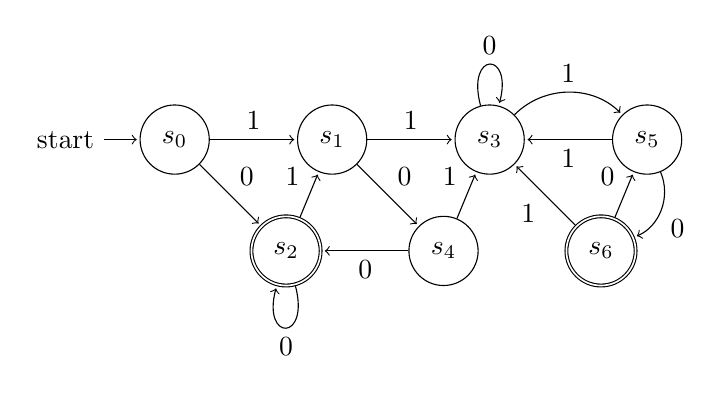
\begin{tikzpicture}[shorten >=1pt,node distance=2cm,on grid,auto] 
   \node[state,initial] (s_0)   {$s_0$}; 
   \node[state] (s_1) [right=of s_0] {$s_1$}; 
   \node[state,accepting] (s_2) [below right=of s_0] {$s_2$}; 
   \node[state](s_3) [right=of s_1] {$s_3$};
   \node[state] (s_4) [below right=of s_1] {$s_4$}; 
   \node[state] (s_5) [right=of s_3] {$s_5$}; 
   \node[state,accepting] (s_6) [below right=of s_3] {$s_6$}; 
    \path[->] 
    (s_0) edge  node {1} (s_1)
          edge  node {0} (s_2)
    (s_1) edge  node {1} (s_3)
          edge  node {0} (s_4)
    (s_2) edge  node {1} (s_1) 
          edge [loop below] node {0} ()
    (s_3) edge [loop above] node {0} ()
	      edge [bend left=45] node{1} (s_5) 
    (s_4) edge node {1} (s_3)
		  edge node {0} (s_2)
    (s_5) edge node{1} (s_3)
	      edge [bend left =45] node{0} (s_6)
    (s_6) edge node {0} (s_5)
          edge node {1} (s_3);     
\end{tikzpicture}



Consider the Finite State Automaton $A$ drawn above.\\

(a) Find the 0,1,2, and 3- equivalence classes of states of $A$.\\

Solution: The 0-equivalence classes are easy:
\[
\{s_0,s_1,s_3,s_4,s_5\} \text{ are the nonaccepting states}
\]
\[
\{s_2,s_6\} \text{ are the accepting states}
\]

For the 1-equivalences, let's look at the accepting states first.  $s_2$ is 0-equivalent to $s_6$ but $N(s_0,0)$ is not 0-equivalent to $N(s_6,0)$ so these are not 1-equivalent.  So far we have
\[
\{s_2\},\{s_6\}
\]

Now let's look at the nonaccepting states.  First, let's consider $N(s_j,0)$  in this case, only $s_0,s_4,s_5$ go to accepting states, whereas $N(s_1,0),N(s_3,0)$ are nonaccepting states.  Now considering $N(s_j,1)$ we see that $s_0,s_4,s_5$ all go to nonaccepting states and so they form a 1-equivalence class.  Finally, $N(s_1,1)$ and $N(s_3,1)$ go to nonaccepting states.  This leaves us with the 1-equivalence classes:
\[
\{s_0,s_4,s_5\},\{s_1,s_3\},\{s_2\},\{s_6\}
\]


Now let's consider the 2-equivalence classes.  $s_2$ and $s_6$ are their own classes, and so there is nothing left to test there.  Now let's test $s_1$ against $s_3$.
\[
s_1 R_1 s_3
\]

We need to check whether or not the two following statements are true
\[
N(s_1,0) R_1 N(s_3,0)
\]
\[
N(s_1,1) R_1 N(s_3,1)
\]
We see that these are not true since
\[
s_4 = N(s_1,0) \not{R}_1 N(s_3,0) = s_3
\]

Now we check the triple $\{s_0,s_4,s_5\}$.

We need to compute the following:
\begin{eqnarray}
N(s_0,0) & = & s_2 \nonumber \\
N(s_0,1) & = & s_1\nonumber \\ 
N(s_4,0) & = & s_2 \nonumber \\
N(s_4,1) & = & s_3\nonumber \\ 
N(s_5,0) & = & s_6 \nonumber \\
N(s_5,1) & = & s_3\nonumber  
\end{eqnarray}

Checking all of these things we get the 2-equivalence classes

\[
\{s_0,s_4\},\{s_1\},\{s_2\},\{s_3\},\{s_5\},\{s_6\}
\]

In the three equivalence classes, we only need to check $\{s_0,s_4\}$.

We have
\[
s_0 R_2 s_4, \text{ and } N(s_0,0) R_2 N(s_4,0)
\]

However we falter at
\[
s_1 = N(s_0,1) \not{R}_2 N(s_4,1) = s_3
\]

(b) Draw the transition diagram for $\bar{A}$, the quotient automaton of $A$.

The $*$ equivalence classes are the singular states, so the diagram above is the quotient machine.


\newpage

\section{Notes}

\S 2
The first problem in this assignment is a special case of Stirling's approximation.  In truth, the denominators $2^n$ and $3^n$ converge on $e^n$.  This fact can be derived from the fact that
\[
\lim_{n\rightarrow \infty} \left(1 + \frac{1}{n}\right)^n = e.
\]

By many estimations is it $e$ rather than $\pi$ which is the most important irrational number.  That is a matter of opinion, but those holding that opinion are certainly not without their reasons. A couple more related pieces of information about $e$ and $\pi$ and Stirling's approximation.
\[
e^{i\pi}+1 = 0
\]
This is said to contain the five most important numbers in all of the sciences.

A stronger form of Stirling's approximation tells us when $n$ gets large ($6.02\times 10^{23}$) or so:
\[
n! \approx \frac{n^n}{e^n} \implies \ln(n!) \approx n\ln(n)-n
\]

This is an extremely widely used fact in both algorithm analysis and statistical mechanics/statistical thermodynamics.  However, we can prove it by induction.  The strongest form, however is:
\[
\lim_{n\rightarrow\infty} \frac{n!e^n}{n^n\sqrt{n}} =\sqrt{2\pi}
\]

Again we see $\pi$ showing up.\\

The second problem is Fermat's little theorem.  This little gem allows us to factor some polynomials a little more easily, and since we know squaring and cubing, etc keeps integer parity (even to even, odd to odd) we can actually prove additional facts such as:
\[
6|(n^3-n), \text{ and } 10|(n^5-n)
\]

We'll see this fact again when we begin talking about prime testing integers.  Testing integers for primality is a relatively ``fast process," but factoring them still takes quite a while, especially if they're about the size of public key encryption keys ($10^{600}$ or so).

Problems three and four are fairly standard induction type problems.  Problem five is where we get some interest.  These $(\lambda, v)$ pairs are called eigenvalue, eigenvector pairs.  ``Eigen" is German (and Dutch) for characteristic of, or self.  The multiplication we see in parts (c) and (e) is called the eigen decomposition of a matrix.  The way we compute eigenvalues is to take the determinant of the matrix $L-\lambda I$.  Since this is a function of $\lambda$ we solve the particular $\lambda$s for which this becomes zero.
\[
\det(L-\lambda I) = 0.
\]

If you haven't had linear algebra yet, you'll need to look up the determinant of a matrix, but in the end, it becomes a polynomial.  In fact, perhaps not surprisingly it's called the ``characteristic polynomial" of a matrix.  Eigenvalues and eigenvectors have approximately infinitely many uses to the best of my knowledge.  Interestingly enough, in physics they are used to measure energies of quantum systems, and in fact they end up being the probabilities on which we base our measurements in a quantum computer.  They show up in modeling fluid mechanics, graph search problems, stereochemistry, and roughly $10^{23}$ more types of sciences.  The study of such properties of matrices arising from graphs is called spectral graph theory (spectrum in this case means the set of eigenvalues).  We use this to produce probabilistic results for walks on graphs.  This is more or less the technique used by tech giants to give ``relevant search results."  The Laplacian of a graph is also used to make ``quantum random walks" which behave quite strangely, but the mathematics is the same as we've just seen.  We simply compute:
\[
e^{-itL}
\]

And look at its properties.\\

\par Earlier we had mentioned that we can compute $f(L)$ for well behaved things.  Here, by ``well-behaved" we mean any $n\times n$ matrix with $n$ distinct eigenvalues, or $n$ linearly independent eigenvectors (again, you'll want to look up linear independence, although it comes up later in this course in a different context).  Additionally, we need the function $f$ to converge to its Taylor series.  Yes, THAT Taylor series, from calculus.  If all these criteria are satisfied (sufficient, but not necessary, ie there are a few additional cases that work) then we can compute $f(M)$ by
\[
f(M) = Pf(D)P^{-1}
\]
where $P$ is the matrix with eigenvectors as columns and $D$ is the diagonal matrix with the eigenvalues on the diagonal.  This technique is called functional calculus (or in some cases, spectral calculus).

\S3
Pell's equation is interesting in that it is an approximation algorithm to find good approximations for square roots.  Once we have the fundmental solution (or any solution for that matter) we can calculate a good approximation for $\sqrt{n}$ relatively quickly since $(x_k,y_k)$ are growing quite fast.  This means:
\[
(x_k - \sqrt{n}y_k) = \frac{1}{(x_k+\sqrt{n}y_k)} \approx 0
\]

That tells us
\[
x_k \approx \sqrt{n} y_k
\]

Additionally, think about how we can use the eigenvalue decomposition to compute
\[
\begin{bmatrix}
x_1 & ny_1\\
y_1 & x_1
\end{bmatrix}^k
\]


\par Moving onto recurrence relations, let's just mention some of the things we can move around.  We'll leave out nonlinear equations entirely, but we can have repeated roots, complex roots, higher orders, and nonhomogeneities.  Higher orders are tackled in exactly the same way as second order equations, with more difficult characteristic polynomials.  We touched briefly in the exercises on repeated roots.  In higher order equations, for every time we repeat a root we add a power of $n$.  For example, suppose the characteristic polynomial of a fourth order equation can be factored as
\[
(r-2)^4
\]
then our general solution becomes
\[
a_n = (A+Bn+Cn^2+Dn^3)2^n
\]

In the case of complex roots we have oscillatory solutions.  Consider for example:
\[
a_{n+2}+4a_n = 0.
\]
The roots are $\pm 2i$.
This gives a general solution:
\[
a_n = C(2i)^n + D(-2i)^n
\]
which we can rewrite as
\[
a_n = C(2^n e^{i\pi n})+ D(2^ne^{-i\pi n})
\]
Which gives
\[
a_n = 2^n(F\cos(\pi n)+ G \sin(\pi n))
\]

The Catalan numbers represent the number of ways you can arrange $n$ sets of closed parentheses. For example:
\[
C_3 = 5 \text{ with these five sets } ()()(),(())(),()(()),(()()),((()))
\]

One of the more interesting ways to solve them, which we do not have time to cover in this class is with generating functions.  We define the ordinary generating function of a sequence by
\[
A(x) = \sum_{n=0}^{\infty} a_n x^n
\]

The Catalan numbers converge to a particular interesting generating function.

\[
C(x) = \frac{1-\sqrt{1-4x}}{2x}
\]

Finally, we have a good asymptotic approximation for the Catalan numbers:

\[
C_n \sim \frac{4^n}{n^{3/2}\sqrt{\pi}}
\]

The major method for proving this asymptotic formula is Stirling's approximation.  See you if can prove this on your own.


\S4

The relations $D$ and $D_k$ that we've defined in problem 2 lead us into some very interesting territory that we'll begin exploring next week.  In particular, we can offer a proof for the quotient remainder theorem using $D$.  However, this is not so exciting.  We will define new operations on the equivalence classes of $D$ and via this we will be able to define modular arithmetic.  We'll also be able to move into discrete logarithms, chinese remainder theorem, and ``fast" methods for testing primality.  All of these together lead us into the famed RSA encryption.  The truth of the matter is that we can really build this technology on the back of the equivalence relations we've defined in problem 2.

\par Problem 3 gives us a more geometric interpretation of equivalence relations on the integer plane.  $R_{1,1}$ as we wrote it is the set of constant differences.  It is similar to defining rational numbers via an equivalence relation which we will see in class.  What do geometric significance to $n$ and $m$ have?

\par Problem 4 gives a new spin to an old graph theoretic equivalence relation, connected components.  With our new definitions, it is MUCH easier to define connected components.  In this can, the connectivity is slightly offset by one step.  This dramatically changes the equivalence classes.  In a more proper notation, let $A$ be the adjacency matrix of $G$.
\[
vTw \iff \exists k\in\mathbb{N} \text{ s.t. } A^{2k}_{v,w}\ne 0
\]
How is this equivalence relation related to Eulerian and Hamiltonian circuits?  Think about how easy it is to add a single edge to a graph and merge two equivalence classes.  Basically, we just add a diagonal edge across a square connecting two vertices which were in separate classes.  This allows us to reach with an even number of steps all the vertices which previously required an odd number of steps.  Why doesn't this relation produce more classes if we consider longer length walks?

\par In addition to all of these uses for equivalence classes; the field of topology.  There are objects called vector bundles in mathematics and physics.  These objects are basically enormous geometric spaces in which there is a base geometric object, a sphere for example, and attached to every point of that object is a copy of $\R^n$ for some $n$.  The way that we make sense of these vector bundles is to define the set of a bunch of copies of $\R^n$ related to each other by some equivalence relation, which tells us how to glue them together in some coherent way.  This is the basis of GPS systems and how they make sense of maps on the surface of the earth.  In this case, to every point on the globe we glue a copy of the plane $\R^2$ and we decide what it means to move from one point to another via an equivalence relation.  That being said, generally relatively (yes, Einstein's big theory) gives us a recipe for how to glue space together via an equivalence relation. 

\S5

This homework gives us a warm up to showing how public key encryption works.  The first few problems give us different techniques in computing with modular arithmetic.  We have a couple divisibility problems, one of which we have previously solved inductively via two different methods.  Then we move into inverse finding.  It is important to  note that finding an inverse $y$ of $x\mod{n}$ is possible only when $\gcd(x,n)=1$

\[
\exists y\in \Z/n\Z \text{ s.t. } xy\equiv 1\mod{n} \iff \gcd(x,n)=1.
\]

We also move into solving arbitrary problem modulo $n$.  In this case we have
\[
xy\equiv 1\mod{n} \implies x(yk) \equiv k \mod{n}
\]

In some cases we can find $z$ so that
\[
xz\equiv k \mod{n}
\]
but when $x$ is invertible we can solve this equation for arbitrary $k$.  We take a slightly more complicated approach when looking at discrete logarithms.  One approach to solving discrete logarithms is to try brute force search, but this takes an absurdly long time even for relatively small $n$.  For example solving 
\[
3^x \equiv 5 \mod{101}
\]
requires a lot of time to solve by hand.  If we had chosen $n=1001$ this problem becomes almost intractable by hand.  The trick is to realize
\[
a^{100}\equiv 1\mod{101}
\]

Which says is $a^k\equiv1$ then $k|100$. So we look at the quantities $3^2,3^5,3^{10},3^{25},3^{50}$.  If none of those are 1 then we can solve an arbitrary problem.  The smallest number $k$ so that
\[
a^k \equiv 1 \mod{n}
\]
is called the period of $a$.  Shor's algorithm, which is the quantum algorithm that gets so much attention, relies solely on the fact that a quantum computer can solve discrete logarithms faster than digital computers.  The rest of the factorization is already easy to compute on digital computers.

\par  Once we've moved in that direction, we build our own public key encryption. We distribute $(n,e)$ publicly.   Given this information, one may assume that decrypting this by finding $d$ is easy.  The reason that this information is secure is because even given a public key $(n,e)$ computing the correct $d$ is difficult.  So difficult in fact, that even with the best technology we have, the amount of time it takes to compute $d$ is exponential in the number of bits of $n$.  When $p$ and $q$ have 500 digits each, $n\sim 10^{1000} \sim 2^{3322}$.  With more than 3300 bits of information, $e^{3300}$ is unfathomably large.\\ 


\par Just as a point of information, it may help you to remember how to construct ann encrytpion scheme by remembering: $M$ is for message, $e$ is for encryption, $d$ is for decryption, and $C$ is for cypher.


\S6

We're getting the techniques together so that we can start analyzing the runtime analysis of algorithms.  We've also studied some pieces that are related to other incredibly important algorithms in numerical analysis.  In problem one, we see the Chinese Remainder Theorem.  One sufficient condition for solving the Chinese Remainder theorem is if $\gcd(n_j,n_k)=1$ in
\[
x \equiv a_i \mod n_i
\]

That is, every pair of moduli are mutually prime.  In the early parts of abstract algebra we learn that there is a set isomorphism (a bijective function between sets which also preserve extra structures like addition) given by

\[
\Z /N \simeq \prod_{p|N} \Z/p
\]

Moving into problem 2 we start seeing faster methods for prime testing.  In truth these prime tests are logarithmic in that, each step we reduce the overall number by a factor of ten (order of magnitude).  So if a number $N$ is of order $10^7$ we must perform at most 7 iterations of two digit multiplication and a subtraction.  This means, we require $2\log_{10}(N)$ number of elementary operations to check each prime.  Additionally, we know we only have to check all the primes up to $\sqrt{N}$ to check whether or not $N$ is prime.  This tells us, we need approximately
\[
2\phi(\sqrt{N}) \log_{10}(N)
\]
operations to check primality of $N$.  Relatively speaking, this is a huge speedup.  For example, to check whether $N\approx 10^9$ is prime we need
\[
2*(10^{3.5})*9 \approx 18000
\]
steps to check the primality of a number in the billions!

Problem 3 are two small applications of geometric sums which we proved way back in homework 1.  Part b is particularly important as it shows up in solutions to differential equations modeling all manner of things.  Another use for the primitive roots of unity is in Fourier transforms, continuous and discrete.  The discrete transform is an $N\times N$ matrix given by

\[
\mathcal{F}_{jk} = \frac{1}{\sqrt{N}} \omega^{jk}
\]
In truth though, we only really consider
\[
\omega^{jk \mod{N}}
\]
What's the point of computing $\omega^{500}$ when $\omega^8 = 1$.  These points $\omega^j$ in the complex plane are evenly spaced around a circle of radius 1.\\  

\par Problem 4 is the classical part of Shor's algorithm.  The difficult part, as we have seen in computing discrete logarithms.  Once we have found such a $t$ which satisfies $a^t \equiv 1$ then factoring becomes ``easy" in the sense that it can be done by an old slow computer running an old version of java in a matter of minutes.


\S7

There is a lot to say about function complexity, but for this particular assignment we're just getting the hang of analyzing the growth of functions.  Among the most interesting ideas in this homework, in my opinion, are the relations defined in problem 5 where we can make the analogy from relations on functions to relations on numbers via
\[
O \leftrightarrow \le, \Omega \leftrightarrow \ge, \Theta \leftrightarrow =
\]

There are other relations which are similar but we remove the reflexivity called ``little-o" and ``little-$\omega$."  Most of our analysis relies on the fact that we're dealing with enormous numbers, for example we're trying to organize a terabyte of data.  That's a lot of pieces of information.  However, in physics and engineering, we use $O$ as approximations near 0.  For example, the classic approximation for $\sin(x)$ (where $x$ is in radians) is
\[
\sin(x) = \sum_{n=0}^{\infty} \frac{(-1)^n x^{2n+1}}{(2n+1)!} = x - x^3/6 + O(x^5) 
\]

when $x$ is small we reduce computing an infinite sum to computing a polynomial of two terms.  This is the approximation used is computing the position of a pendulum. 
\[
x= 0.1 \implies x^3/6 = .00016 \text{ and } x^5/120 < 10^{-7}
\]
the third piece of the this approximation adds less than one part in ten million.  Any reasonable approximation (for a large scale phenomenon) will be less accurate then one in ten million, so this can be attributed to measurement error.  How accurately to we measure height, weight, age?  Certainly we don't measure height with micrometer accuracy, not weight to the $1/1000$ of a pound, nor age to the millisecond?  How accurate are nails on the wall when we hang pictures?  My guess is that even the most diligent and anally retentive interior decorator is off by a few thousandths of an inch and that's $10^{-3}$.  No need to be 10000 times better than that!  It is this ability to accept error that allows us to speed up our algorithms tremendously!  For example, consider computing a square root (via the binomial theorem)
\[
\sqrt{1+x} = 1 + \frac{x}{2} - \frac{x^2}{8} + \frac{x^3}{48} - \frac{5x^4}{128} + O(x^5)
\]

We can cut this off after $x^2/8$ when $x$ is small.  Think of the difference in programing a computer to compute the value of a polynomial with 4 terms versus calculating an actual square root.  In the same spirit this is the kind of thinking that allows us to write ``faster" algorithms when we're willing to accept an $O(n^2)$ speed instead of
$O(n^{2-\varepsilon}\log(n)^k)$.  The overall run time may be slightly longer, but we probably save that much time in writing a simpler code which is just slightly less optimized. 

\S8

In most computer science texts the sequence $a_n$ becomes a function on the natural numbers.
\[
a_n \rightsquigarrow T(n) = cT(n/b)+f(n)
\]

In physics we call $f(n)$ the driving force.  This term makes some good sense here in that every recursive call forces us to implement the function $f$ with a smaller input.  In physics when $f$ is the same function as the homogeneous solution then we have resonance or feedback.  In this case, the master theorem tells us that we multiply the overall sorting statistic by an additional logarithmic factor.  In physics the extra factor is either linear or exponential depending on the context of the problem.  When studying recurrence relations back in week three we didn't deal with logarithmic functions, simply exponential ones.  Notice though, that if we were clever about how we indexed our sequences we would be able to come up with nearly identical results.  If you don't believer this go through Cormen et al's proof of the master theorem.  Think about how we would modify a recurrence relation in general for a recursive call of the form
\[
T(n) = cT(g(n))+ f(n) 
\] 

where $g(n)$ is sublinear, that is
\[
g(n)\in O(n) \text{, but } g(n)\notin \Theta(n)
\]

This could be $\sqrt{n}$ or $n^{s}$ with $s<1$.  The master method still works, but it requires a little bit of clever manipulation to get there.

\par Moving into the bulk of the problem set we take a good look at quicksort.  Interestingly, if the array is ``balanced" then the algorithm works in optimal time.  When the array is unbalanced, for example
\[
[10,1,9,2,8,3,7,4,6,5]
\]
quicksort requires approximately $n^2$ operations to complete.  In order to ensure we always get a balanced list we could scan each (sub)array to find the median.  This takes on average $n/2$ tests, then pick this item to sort.  This costs us a little time, but it's not atrocious.  Interestingly, even if we cut  a badly unbalanced array, as long as there is some measurable percentage on either side of the test element, this algorithm runs in $O(n\log(n))$ time.  The constant out front will change, but since we can ``throw away" constants we maintain our asymptotic complexity.  The true recursion looks something like
\[
T(n) = T(q) + T(n-q-1) + (n-1)
\]

where $q$ is the first item in the (sub)array.  Merge sort and heap sort (in binary trees) ensure that we cut every subarray in half, thus leaving us with the recurrence in problem 2.  How would this sorting efficiency change if we used ternary trees rather than binary?  One of the things that makes quicksort so efficient in practice is that it is a sorting algorithm which is ``in place."  This means we only ever never a constant amount of additional memory spots allocated to help with the switches.  So while it may have a slow run time, this is very rare if we're given a ``random" sequence.  In terms of space as a resource, quicksort is as efficient as it gets!

\par Stooge sort is new to me.  It's terribly inefficient, but as you've probably already discovered, it does, in fact, get the job done correctly.  It just take a LONG time (relatively speaking). How could you modify this to take even longer, but still ensure the correct run time?  What is the exponent on that runtime?  It appears that all sorting algorithms which have a bounded runtime (bogosort doesn't actually sort) are still algebraic, vs the runtime to solve a Towers of Hanoi puzzle. 

\S9
Throughout the two quarter we have just completed, we have talked about the theory of computing in several ways.  Some direct i.e. logic and truth tables, and some indirect i.e. modular arithmetic.  Most of the work we've talked about, however is binary logic based.  This theory of computation is incredibly as we have seen, but logical gates have ``no memory."  Finite state automata (or finite state machines) have some amount of ``memory."  That it to say, that if we're operating a vending machine, and we want to get a small item which costs \$1.  We shouldn't have to put in only \$1 coins.  We should be able to add dimes and quarters as well.  The finite state machine is capable of ``remembering" how much money we've put into the machine.  When you go further into the theory of computation you will begin studying Turing Machines.  You will find the definition of Turing Machines similar to that of finite state machines, with the addition of a memory tape.  Turing machines, therefore, have ``unlimited" memory.  The Church-Turing thesis tells us that anything which is ``computable" can be computed by some Turing machine.  It is this definition which tells us what is and is not computable.  Moving forward in time we will begin using different types of machine, be they molecular computers, DNA computers, quantum computers, or some hybrid of all of the above, these new architectures may be able to do all sorts of new computations, but that's a little bit inaccurate.  In truth, building a computer on a new architecture may be able to improve  the speed by which we compute things, but it should not give us new computable objects.  The objects we're talking about which are ``newly computable" are simply things which have become tractable.  That is, these things can now be computed in a ``reasonable" amount of time (polynomial in the size of the input) rather than in the age of a million universes (exponential or superexponential in the size of the input).

Notice that finite state automata are able to compute binary logical operations by allowing a two symbol alphabet.  In order to compute ternary or $n$-ary logic we simply need to design a finite state machine with an input alphabet of 3 or $n$ symbols.  

It should come as no surprise to us that Kleene was both one of the main promoters of 3 valued logic and one of the main figures in defining formal languages.  His 3 valued logic was based on a three symbol alphabet
\[
\Sigma = \{1,0,-1 \} \simeq \{T,U,F\}
\]
Let's recall our quick calculation from the beginning of Discrete Math 1.  Given $n$ variables in $|\Sigma|$ values we have
\[
|\Sigma|^{|\Sigma|^n} 
\]
possible gates/computations.  As the size of the alphabet, $\Sigma$ grows, the number of computable problems grows superexponentially.



\end{document}

